\documentclass{article}
\usepackage{graphicx}

\begin{document}
\title{Design of the Search \& Rescue Bots Project \\
       Artificial Intelligence~II}
\author{Anton Rebgun \and Dimitri Zarzhitsky}
\maketitle

\section{Objectives}
To build a flexible framework suitable for experimenting with the AI~II concepts using a problem of autonomous micro-aerial vehicles (MAVs) attempting to locate fires in buildings after a natural disaster, such as an earthquake.  The framework is to be written in Java to facilitate portability, to provide a GUI, to simplify experimentation, and to include a programmer's manual, suitable for later developments of the source code base.

\section{Basic Overview}
The first attempt follows the ``keep it simple'' strategy, hence we make the following assumptions:

\begin{itemize}
\item The simulation uses lock-step time, meaning all events, such as MAV movement, take place in a synchronous fashion.

\item There exists a world object that keeps track of the maps of the environment, location of the MAVs, and the building fires.  The maps follow a layered structure, which allows to keep some things, such as the map of the buildings' location static.

\item We assume that MAVs are dimensionless, and hence will not address collision handling in the first version of the simulator.
 
\item The first version will also assume an infinite supply of fuel, hence the number of MAVs will remain constant throughout the simulation run (we're assuming that an MAV cannot be damaged or otherwise disabled).  This restriction will be relaxed in the subsequent version of our program.

\item The simulator follows the model-view-controller (MVC) design pattern, where a GUI object will control the World and MAV objects, and also provide a control interface.  If time and resources allow, we will create a ``batch'' mode interface for the system in order to simplify empirical experiments.

\item We will use a basic threading structure to separate the simulator's model and the view-control components to take advantage of computers with multiple CPUs.

\item The code will follow principles of good Object-Oriented design by using Java packages, interfaces, and a possible extensive inheritance hierarchy, which will allow us to first create very simple and rudimentary implementation units, and then allow others to improve on our work in a straightforward fashion.

\item The agent objects will consist of several intrinsic properties, such as the orientation, location, velocity, and a certain amount of available fuel (which will be unlimited in the first version).  The world and agent coordinate systems will be synchronized, that is the agents will make use of ``global'' reference coordinate system, consistent with our expectation that a GPS unit will be available.

\item Agent entities will allow for a set of different world sensors, e.g. sonar, camera, etc, which will query the world object to obtain the pertinent information.  Each sensor will have a specified field of view, varying from a simple circular patter to a more sophisticated Gaussian profile.  The World object will be responsible for updating the dynamic maps, such as those of MAV location and building fires.

\item We plan to make extensive use of the Java {\tt Region} interface, which provides a rich interface of geometric test function to simplify computation of sensor view maps.  Thus the output of each sensor unit is a set of generic polygonal shapes, and we should be able to construct a variety of navigation algorithms using this flexible approach.
\end{itemize}


\subsection{Agent Object}
We anticipate that the agent object will consist of the following generic sub-modules:

\begin{itemize}
\item propulsion unit (first implementation assumes a simple 360-degree thruster with a variable speed output, allowing the unit to move in any direction with some maximum speed).

\item sensor module, where we anticipate the bulk of our work to take place; we envision a sonar-like module and an infrared-base module (for fire detection).  In both cases, these are simple, binary-like sensor units.

\item we will provide a placeholder for a MAV communication module, but will not implement any of the communication foundation in the first version of the simulator.

\item a placeholder planning module will be provided, which in the first version will implement a simple behavior, such as spiraling (combined with reactive obstacle avoidance).

\item if we are successful in implementing the major goals of this project, we will extend it by creating two types of MAV agents: scouting agents, whose responsibility is to maximize sensor coverage of their flight path, and the perching agents whose goals is to observe the maximum number of buildings for possible fires.
\end{itemize}

\subsection{World Object}
The world object is the central data structure of the simulator, which encapsulates the current state of the task, such as location of the MAVs, the buildings, fire, and the general map of the environment.  The World object will provide a rich set of query and modifier functions that will allow for a variety of MAV sensor modules.  However, the World object will not contain any of the program's global structures - that responsibility will be delegated to a more transparent simulator object, which will also serve as the communication point between the viewer-controller (i.e. the GUI) and the rest of the program.


\section*{Appendix}
\begin{figure}[!b]
\centering
\includegraphics[width=\textwidth]{sensor_profiles}
\caption{Envisioned sensor profiles for the MAVs.}
\label{fig:sensor_profiles}
\end{figure}

\begin{figure}
\centering
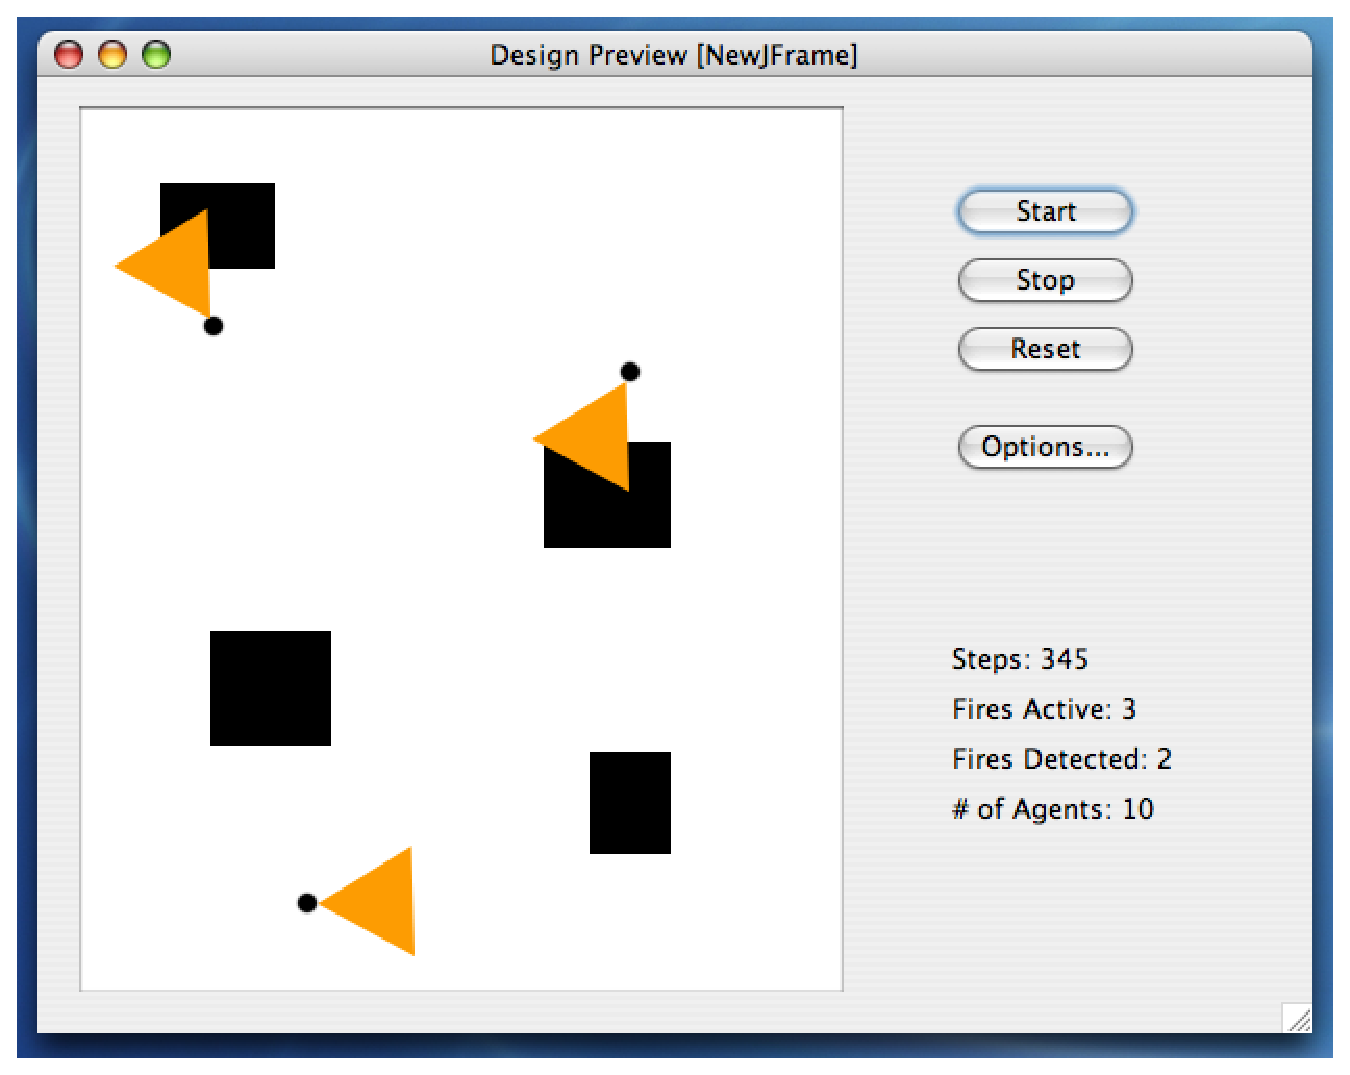
\includegraphics[width=\textwidth]{GUI_mockup}
\caption{GUI prototype.}
\label{fig:sensor_profiles}
\end{figure}

\end{document}

% LocalWords:  Rebgun MAVs MAV MVC GPS
